 %%%%%%%%%%%%%%%%%%%%%%%%%%%%%%%%%%%%%%%%%
% Short Sectioned Assignment LaTeX Template Version 1.0 (5/5/12)
% This template has been downloaded from: http://www.LaTeXTemplates.com
% Original author:  Frits Wenneker (http://www.howtotex.com)
% License: CC BY-NC-SA 3.0 (http://creativecommons.org/licenses/by-nc-sa/3.0/)
%%%%%%%%%%%%%%%%%%%%%%%%%%%%%%%%%%%%%%%%%

%----------------------------------------------------------------------------------------
%	PACKAGES AND OTHER DOCUMENT CONFIGURATIONS
%----------------------------------------------------------------------------------------

\documentclass[paper=a4, fontsize=11pt]{scrartcl} % A4 paper and 11pt font size

% ---- Entrada y salida de texto -----

\usepackage[T1]{fontenc} % Use 8-bit encoding that has 256 glyphs
\usepackage[utf8]{inputenc}
%\usepackage{fourier} % Use the Adobe Utopia font for the document - comment this line to return to the LaTeX default

% ---- Idioma --------

\usepackage[spanish, es-tabla]{babel} % Selecciona el español para palabras introducidas automáticamente, p.ej. "septiembre" en la fecha y especifica que se use la palabra Tabla en vez de Cuadro

% ---- Otros paquetes ----

\usepackage{amsmath,amsfonts,amsthm} % Math packages
%\usepackage{graphics,graphicx, floatrow} %para incluir imágenes y notas en las imágenes
\usepackage{graphics,graphicx, float, url} %para incluir imágenes y colocarlas

% Para hacer tablas comlejas
%\usepackage{multirow}
%\usepackage{threeparttable}
\usepackage{float}


%\usepackage{sectsty} % Allows customizing section commands
%\allsectionsfont{\centering \normalfont\scshape} % Make all sections centered, the default font and small caps

\usepackage{fancyhdr} % Custom headers and footers
\pagestyle{fancyplain} % Makes all pages in the document conform to the custom headers and footers
\fancyhead{} % No page header - if you want one, create it in the same way as the footers below
\fancyfoot[L]{} % Empty left footer
\fancyfoot[C]{} % Empty center footer
\fancyfoot[R]{\thepage} % Page numbering for right footer
\renewcommand{\headrulewidth}{0pt} % Remove header underlines
\renewcommand{\footrulewidth}{0pt} % Remove footer underlines
\setlength{\headheight}{13.6pt} % Customize the height of the header

\numberwithin{equation}{section} % Number equations within sections (i.e. 1.1, 1.2, 2.1, 2.2 instead of 1, 2, 3, 4)
\numberwithin{figure}{section} % Number figures within sections (i.e. 1.1, 1.2, 2.1, 2.2 instead of 1, 2, 3, 4)
\numberwithin{table}{section} % Number tables within sections (i.e. 1.1, 1.2, 2.1, 2.2 instead of 1, 2, 3, 4)

\setlength\parindent{0pt} % Removes all indentation from paragraphs - comment this line for an assignment with lots of text

\newcommand{\horrule}[1]{\rule{\linewidth}{#1}} % Create horizontal rule command with 1 argument of height

 
 \title{	
 	\normalfont \normalsize 
 	\textsc{{\bf Security and Computer System} \\ Informatics Course \\ Lodz University(2016/2017)} \\ [25pt] % Your university, school and/or department name(s)
 	\horrule{0.5pt} \\[0.4cm] % Thin top horizontal rule
 	\huge WireShark \\ % The assignment title
 	\horrule{2pt} \\[0.5cm] % Thick bottom horizontal rule
 }
 
 \author{Iván Sevillano García} % Nombre y apellidos
 
 \date{\normalsize\today} % Incluye la fecha actual
 
 \begin{document}
 	
 	\maketitle % Muestra el Título
 	
 	\newpage %inserta un salto de página
 	
 	\section{Wiresharck: Network Monitoring Tool}
 	
 	Wireshark is a powerfull tool which can show information about the network traffic, which means to see all packages that goes througth your computer. Using this tool you can see some risky information from the users of the network, or detecting an attack to a server. Let's see an example:\\
 	
 	\begin{itemize}
 		\item The scenario will be as it follows. My computer is sharing internet and it has my phone conected. We are going to start sniffing the net traffic(wlan0) and see what my phone is doing...\\
 		
 		\begin{figure}[H]
			\centering
			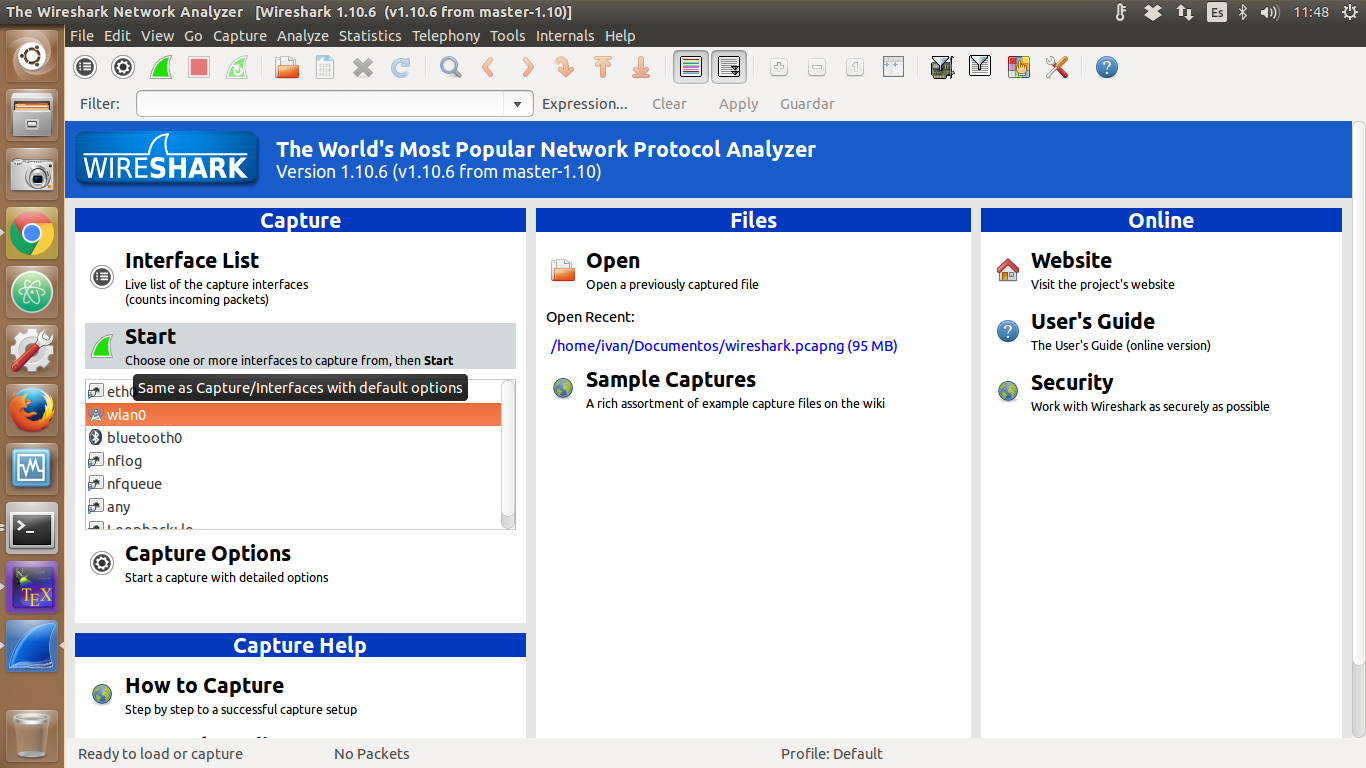
\includegraphics[width=0.7\linewidth]{Wireshark_start_page}
			\caption[Wireshark Start page]{}
			\label{fig:Wireshark_start_page}
		\end{figure}
		
		\begin{figure}[H]
			\centering
			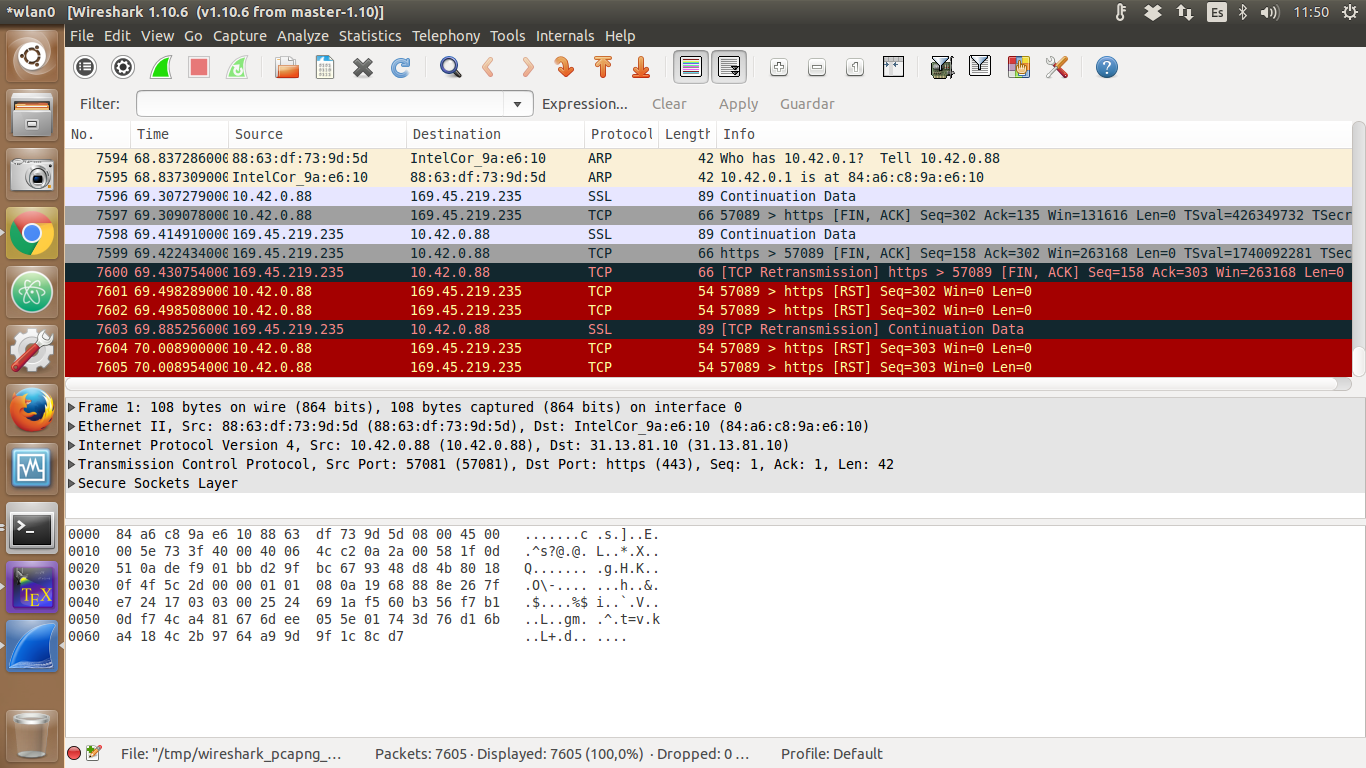
\includegraphics[width=0.7\linewidth]{Wireshark_Sniffing}
			\caption[Sniffed packages]{}
			\label{fig:Wireshark_Sniffing}
		\end{figure}

		\item Now we will see which information could we take. Our network gives directions from 10.42.0.0/24, so we will look for this ips. With a simple nmap scanning, we notice there are three ips connected, one of them is the router(my computer), one of them should be my phone and the other one must be one of my friends phone. We are not going to look for what he is doing, so pay attention to my phone(.32 ip). Also, we want to know what is this phone looking, for example, on internet(http packages):\\
		
		\begin{figure}[H]
			\centering
			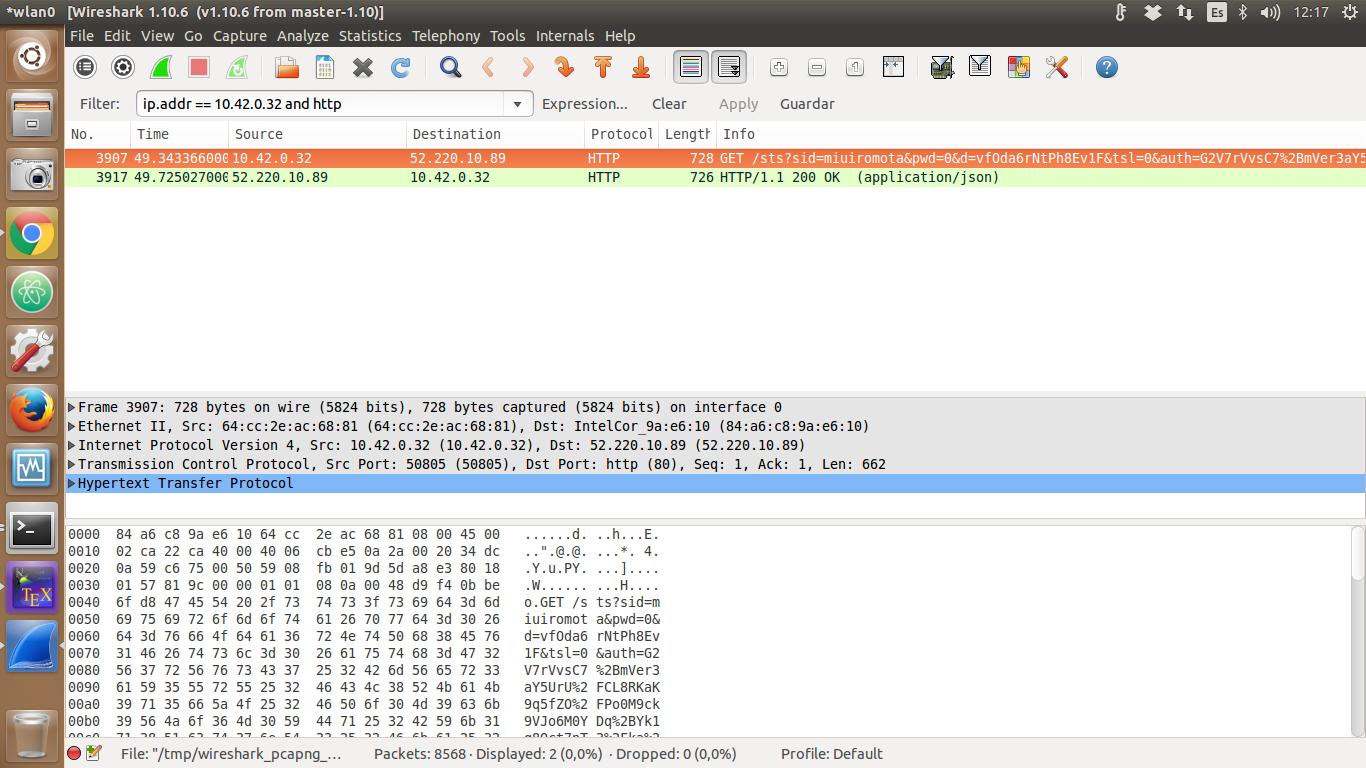
\includegraphics[width=0.7\linewidth]{Wireshark_lookingFor}
			\caption[Wireshark commands]{}
			\label{fig:Wireshark_lookingFor}
		\end{figure}
		
		\item If we follow the TCP Stream of the http package with the "GET" method, that is what we see:\\
		
		\begin{figure}[H]
			\centering
			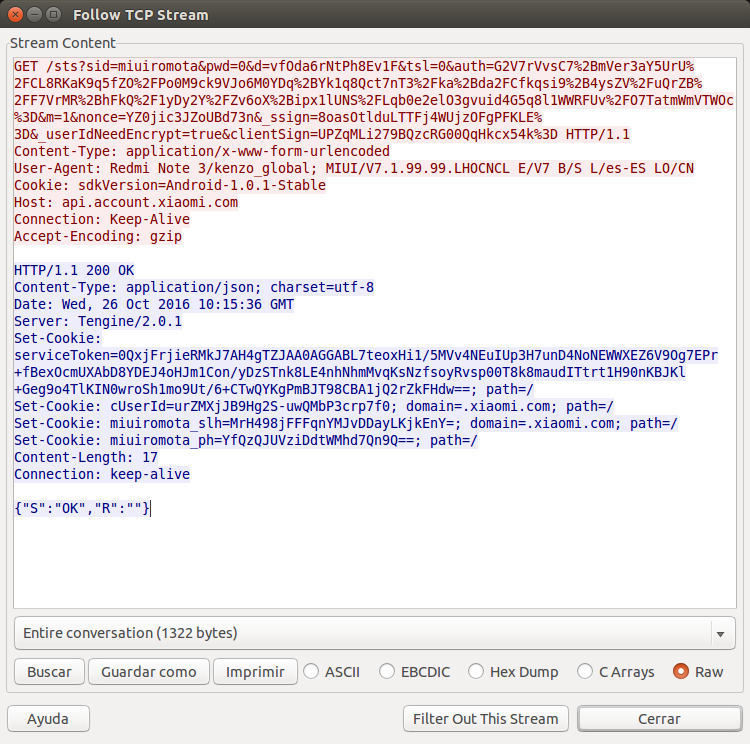
\includegraphics[width=0.7\linewidth]{Wireshark_TCPStream}
			\caption[Wireshark TCP Stream]{}
			\label{fig:Wireshark_TCPStream}
		\end{figure}
		
		\item We can see information of not only the Web page the user has visited, we can also see the user hardware.

 	\end{itemize}
 	
 	That is just like the "Hello World" for Wiresharsk.
 	
 \end{document}